\chapter{Markov Chain Monte Carlo}
\section{Monte Carlo}
Monte Carlo is a general term for computational techniques that use random
numbers.
Monte Carlo can be used in classical and Bayesian statistics. A special kind
of Monte Carlo
called Markov Chain Monte Carlo (MCMC) was one of the main reasons
for the revival of Bayesian statistics in the second half of the 20th century.
Before MCMC became popular, one of the major drawbacks of the Bayesian approach
was that some of the calculations were too hard to do. MCMC enables us to solve
a wide range of Bayesian problems which cannot be solved using analytical
methods.

\subsection{Summaries}
So far, we have represented our probability distributions (prior and posterior)
in a computer by using a vector of possible parameter values and a corresponding
vector of probabilities. For example, suppose we have a single parameter $\theta$
and we have worked out the posterior distribution by using a Bayes' Box. This
will give us a vector {\tt theta} of possible $\theta$ values and a corresponding
vector {\tt post} containing the posterior probabilities. Well, one thing we could
do is plot the posterior distribution, resulting in a plot like the one in
Figure~\ref{fig:normal}.
\begin{verbatim}
plot(theta, post, xlab="Theta", ylab="Posterior Probability")
\end{verbatim}

\begin{figure}[ht!]
\begin{center}
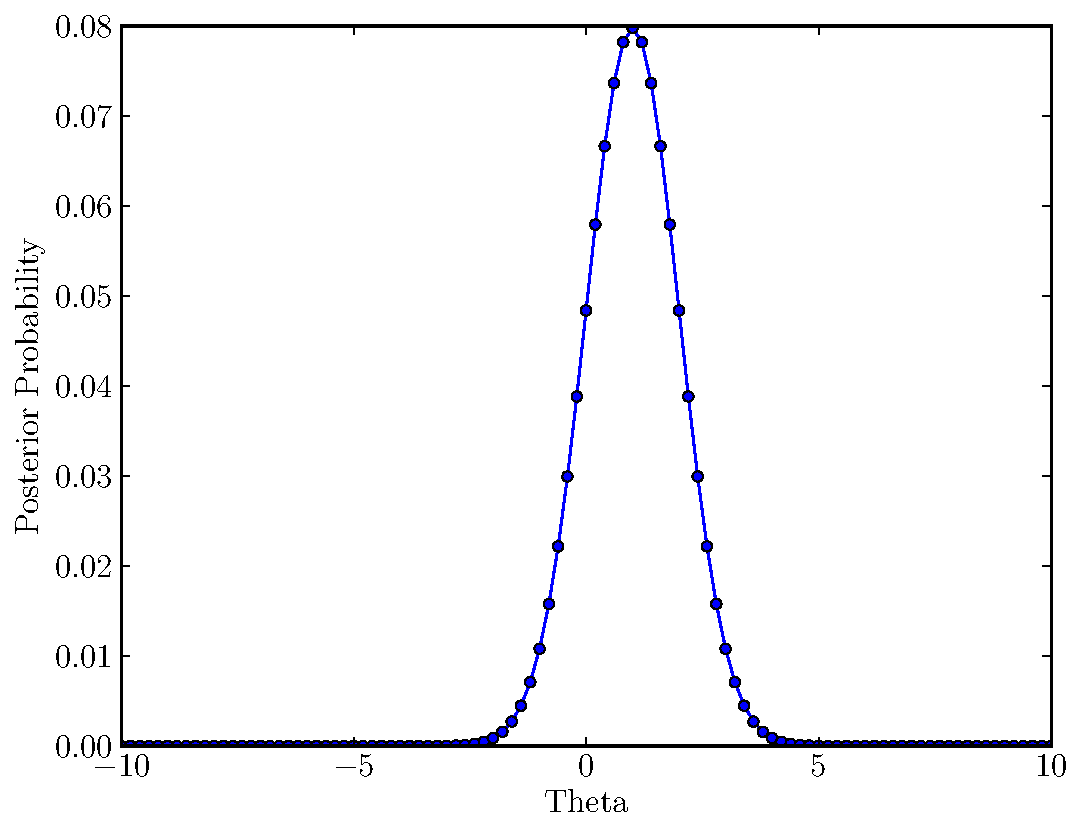
\includegraphics[scale=0.5]{Figures/normal.pdf}
\caption{\it A posterior distribution can be represented in a computer by a discrete
set of possible parameter values, and the corresponding probabilities.\label{fig:normal}}
\end{center}
\end{figure}

If we want to obtain some summaries, we could do it like so:
\begin{verbatim}
post_mean = sum(theta*post)
post_sd = sqrt(sum(theta^2*post) - post_mean^2)
\end{verbatim}

However,
there is an alternative way of representing this posterior distribution in a
computer. It may not be immediately obvious why this is a good idea,
because there is nothing wrong with the tried and true method we have used
so far. But this second method has the advantage that it continues to
work well on much bigger problems, such as when we have more than one parameter.
With more than one parameter, the `vector of possible solutions'' approach
can fail very dramatically.

Our new way of representing a probability distribution in a computer will be
via {\it Monte Carlo} samples.
Instead of having two vectors (one of $\theta$ values and one of the
corresponding probabilities),
imagine we had some method to compute a random sample of $\theta$ values, drawn
from the posterior distribution in Figure~\ref{fig:normal}.
There would only be one vector {\tt theta}. So how would we
know there is greater probability around $\theta=1$? Well, {\it more elements
of the {\tt theta} vector would be near 1}.
Instead of carrying around a second vector of
probabilities, we understand that more probable regions will simply contain
more points. Say our vector of random
samples is called {\tt theta}. Then we can look at the posterior distribution
by plotting a histogram of samples:
\begin{verbatim}
hist(theta, breaks=100)
\end{verbatim}
The histogram looks something like the one in Figure~\ref{fig:normal2}.
\begin{figure}[ht!]
\begin{center}
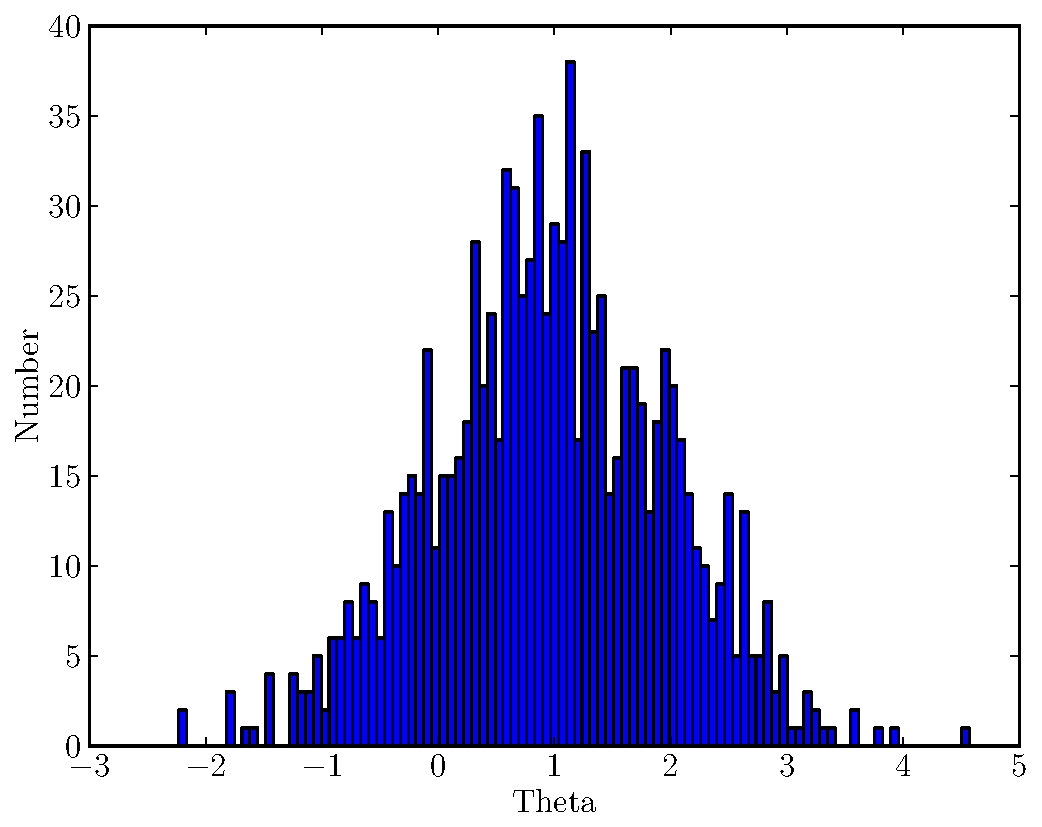
\includegraphics[scale=0.5]{Figures/normal2.pdf}
\caption{\it The posterior distribution for a parameter $\theta$ can also be
represented by a random sample of $\theta$ values drawn from the posterior
distribution. Some $\theta$ values are more probable than others, which is
encoded by certain values appearing more frequently in the sample.
\label{fig:normal2}}
\end{center}
\end{figure}
We can also get our summaries, but the code looks different
(it's actually easier than before!):
\begin{verbatim}
post_mean = mean(theta)
post_sd = sd(theta)
\end{verbatim}
Because of the randomness involved in generating the {\tt theta} values,
the summaries aren't exact. For example, I know the actual posterior mean
and standard deviation in this example were both 1, but the values obtained
from the Monte Carlo samples were 0.9604 and 1.0008, respectively. However,
this doesn't matter much because the results indicate $\theta$ is probably
somewhere around 1, with an uncertainty of about 1. The error introduced by
using random samples is much smaller than the amount of uncertainty inherent
in the posterior distribution itself. For example, if I summarised the posterior
distribution by saying $\theta = 0.9604 \pm 1.0008$, for almost all practical
purposes the conclusion is exactly the same as the true version of the summaries
$\theta = 1 \pm 1$.

In this discussion, we haven't answered the question of how to actually generate
random samples of $\theta$ from the posterior distribution. This is the job
of Markov Chain Monte Carlo.

\begin{framed}
{\bf
The purpose of Markov Chain Monte Carlo is to generate random samples of
parameter values drawn from the posterior distribution. This makes it very easy
to compute summaries even if you have more than one unknown parameter.}
\end{framed}

\section{Multiple Parameters}
MCMC becomes extremely useful when we begin to look at Bayesian models involving
more than one unknown parameter. 
Having posterior samples makes the process of {\it marginalisation}
much easier. Imagine we wanted to infer two parameters, called $a$ and $b$,
from
data $x$. Bayes' rule (parameter estimation version) would give us the posterior
distribution:
\begin{eqnarray}
p(a, b | x) \propto p(a, b)p(x|a,b)
\end{eqnarray}

However, what if you didn't really care about the value of $b$ but
only really wanted to measure $a$? The terminology for this is that $b$ is a
{\it nuisance parameter}: you need it to define the model, but ultimately you
are not really interested in knowing its value.
What you need in this case is the
{\it marginal} posterior distribution for $a$ (that is, the posterior
distribution for $a$ on its own, not the joint distribution with $b$).
This can be obtained using the sum rule. The result is:
\begin{eqnarray}
p(a | x) &=& \int_b p(a, b|x) \, db
\end{eqnarray}
or
\begin{eqnarray}
p(a | x) &=& \sum_{b} p(a, b|x)
\end{eqnarray}
depending on whether the set of possible $b$ values is continuous or discrete.
Before MCMC, these integrals or sums usually couldn't be done without making
certain choices purely for mathematical convenience (e.g. choosing the prior
to be a certain kind of distribution only because it will make the maths work
out, rather than it being a good description of your prior beliefs).

Samples of parameter values drawn from the posterior distribution
(achieved using MCMC) make this hard problem much easier. We no longer need
to worry about mathematical convenience.
See Figure~\ref{fig:marginalisation} for an example showing how Monte Carlo
sampling makes marginalisation trivial.

\begin{figure}[ht!]
\begin{center}
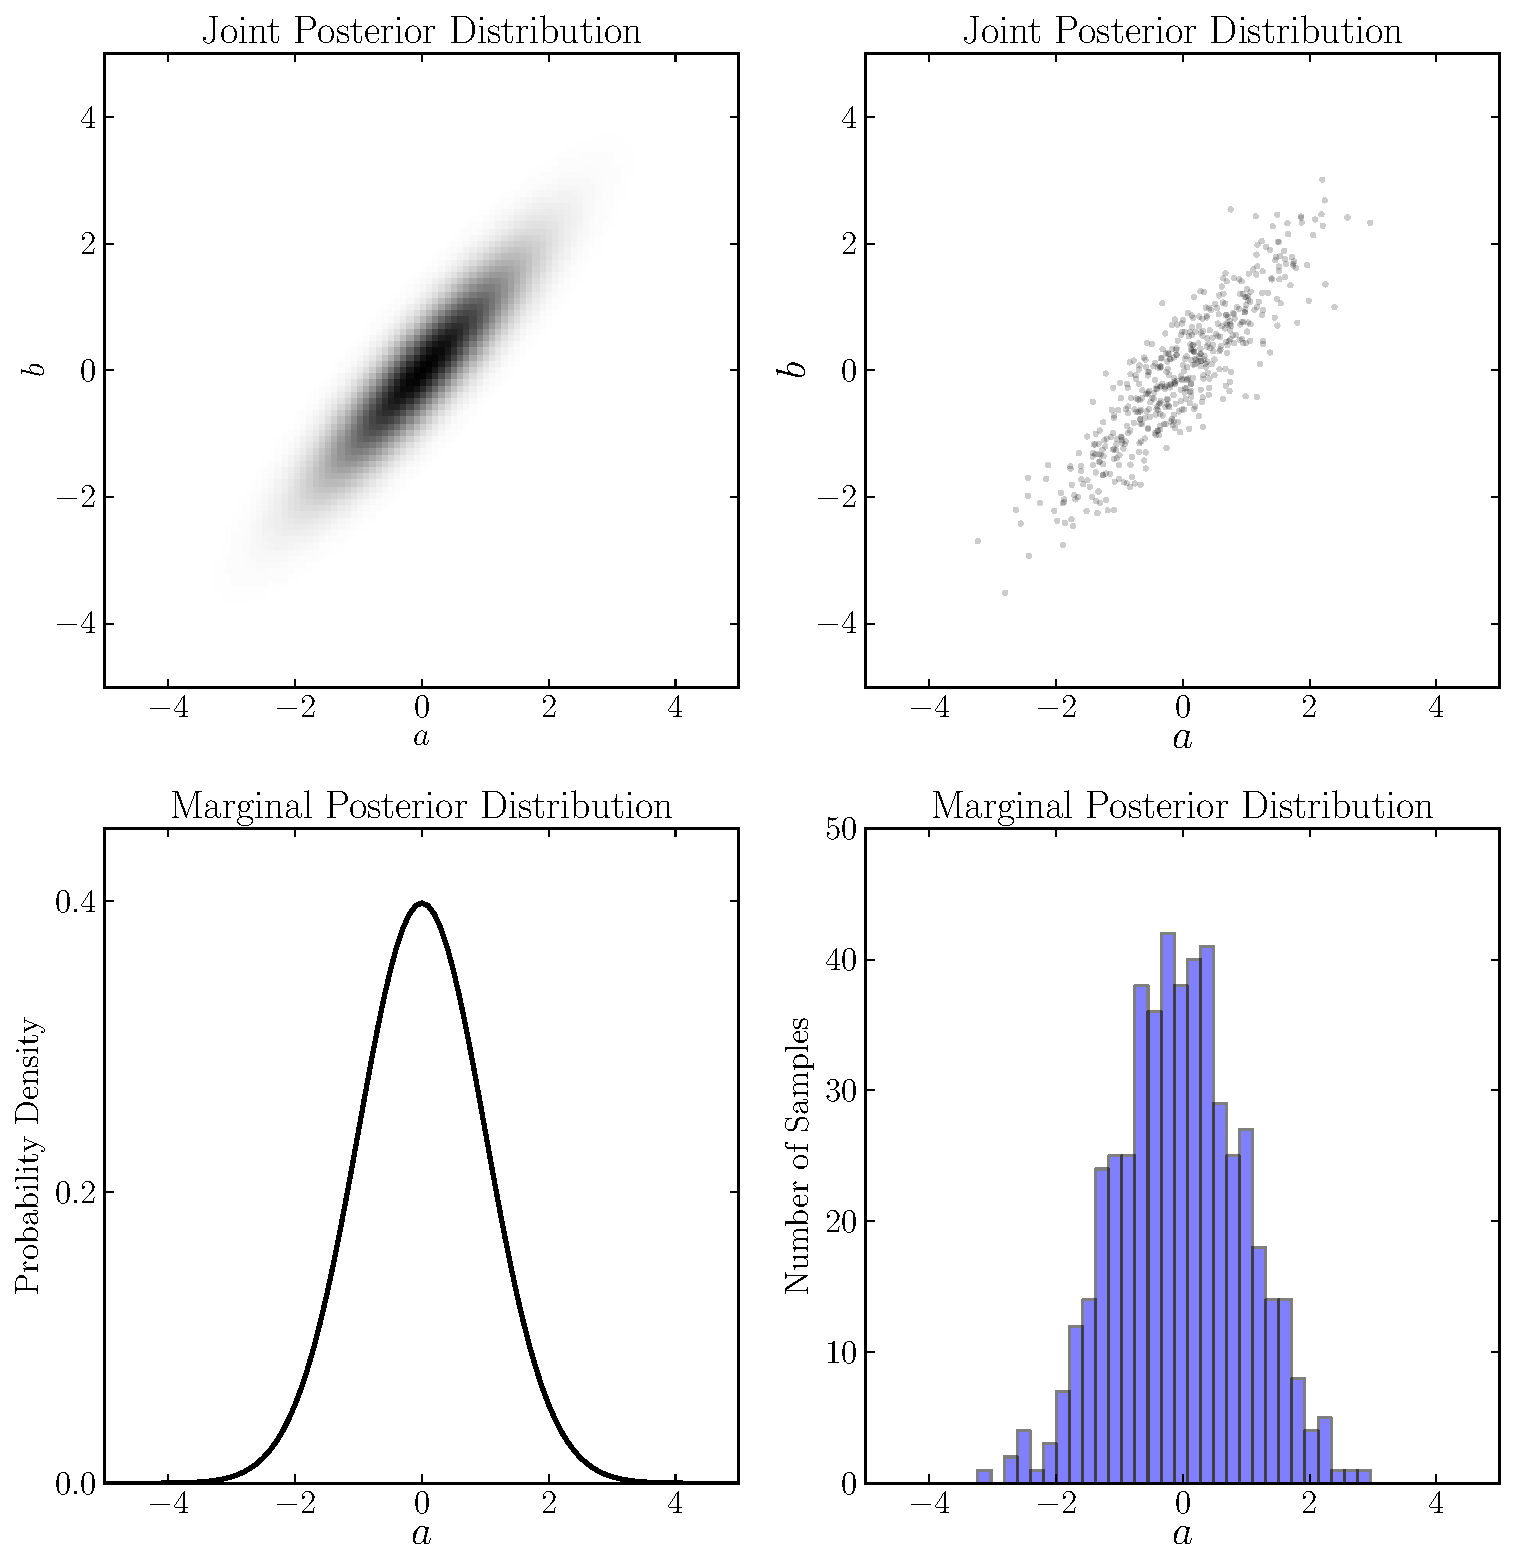
\includegraphics[scale=0.5]{Figures/marginalisation.pdf}
\caption{\it An example of a posterior distribution for two parameters, $a$ and
$b$. The left panels show the joint posterior distribution (which has a
correlation) and the marginal posterior distribution for $a$, obtained by
integrating over all the possible $b$ values. The top right panel contains
random samples
(points) drawn from the posterior distribution for $a$ and $b$.
The only step needed to get the
marginal distribution for $a$ (lower right panel) is to ignore the $b$-values of
the points!
\label{fig:marginalisation}}
\end{center}
\end{figure}


\section{The Metropolis Algorithm}
The Metropolis algorithm is the most basic MCMC method.
The ideas behind it are fairly simple, yet Metropolis forms the basis of a large
number of more advanced MCMC methods. In STATS 331 we will study the basic ideas
behind how the Metropolis algorithm works, which will involve a small amount
of Markov chain theory. We will also look at a small amount of R code
which implements the Metropolis algorithm, but for solving practical problems
it is more convenient to use the JAGS program\footnote{JAGS uses a number
of MCMC methods internally, including Metropolis, ``Gibbs Sampling'', and
``Slice Sampling'', which we will not study in this course.}.

The Metropolis algorithm was invented in the 1950s by physicists
(including Nicholas Metropolis, for whom the algorithm is named), who used it
to do calculations in the field of statistical mechanics. This intriguing field
focuses on calculating the macroscopic (large scale) properties of matter from
knowledge of the small-scale properties. For example, if you know water is
composed of H$_2$O molecules, you can use statistical mechanics to figure out
what will happen if you have a lot
of water molecules. For example, it will freeze at 0 degrees Celsius and boil at 100 degrees Celsius.

It took
many decades before people started to realise the Metropolis algorithm was
useful in Bayesian
statistics as well as statistical mechanics. The Bayesian approach
seemed very elegant and
useful to many people, but it could always be criticised as unworkable,
because you usually had to do difficult or
impossible integrals when solving practical problems
(to summarise the posterior, or to get rid of nuisance
parameters). MCMC changed all that, and is one of the reasons for the
explosion in the popularity of Bayesian statistics beginning in the 1990s.

The basic idea of MCMC is that we want a method which will travel between
different possible states (such as the possible hypotheses/parameter values in
a Bayesian analysis). We want the amount of time spent in
any particular state to be proportional to the posterior probability of the state.
The computer ``explores'' the set of possible parameter values, spending a lot
of time in the regions with high posterior probability, and only rarely visiting regions
of low posterior probability. Figure~\ref{fig:mcmc} shows an example of MCMC
applied to a problem with only two possible hypotheses or parameter values.
Nobody would actually use MCMC on such a small problem, but it is helpful for
explaining how MCMC works.

\begin{figure}[ht!]
\begin{center}
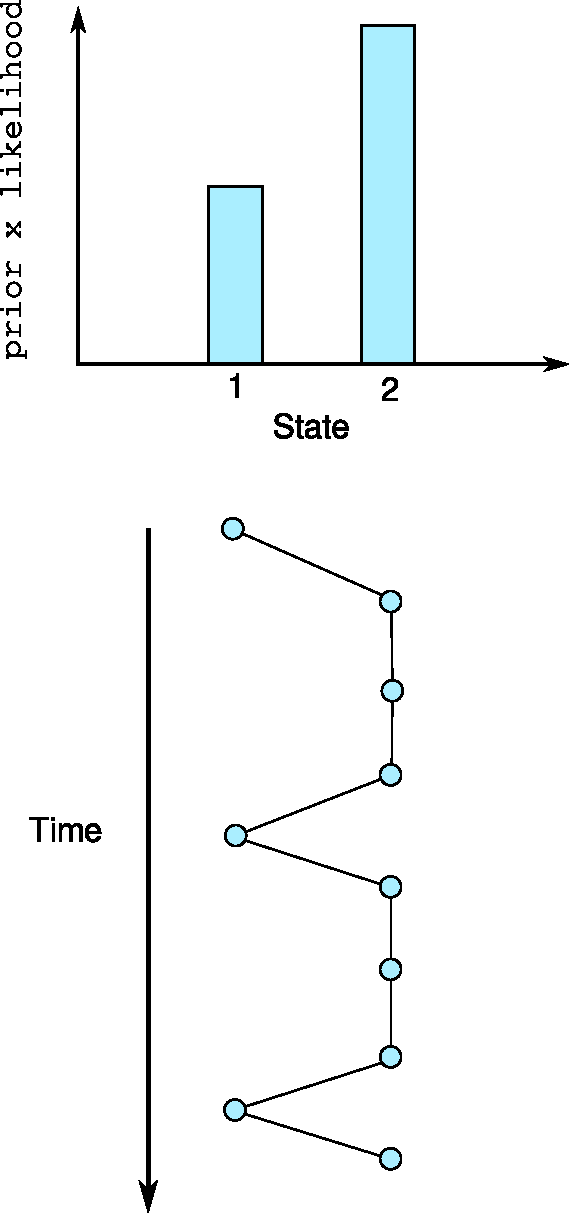
\includegraphics[scale=0.65]{Figures/mcmc.pdf}
\caption{\it An illustration of the basic idea behind MCMC. Imagine we had a
Bayes' Box with two possible hypotheses, and we knew the
{\tt prior $\times$ likelihood} values. The amount of time the MCMC program will
spend in each state is proportional to the posterior probability of the state.
In this example, the MCMC algorithm was in State 1 three times and in State 2
seven times. Using this, we could estimate the posterior probability of State 2
as being 0.7. This estimate would become more accurate if we ran the MCMC for
more iterations.\label{fig:mcmc}}
\end{center}
\end{figure}

\subsection{Metropolis, Stated}
The Metropolis algorithm is given below. The first thing to do is start
{\it somewhere} in the ``parameter space'' (set of possible parameter values).
You then
{\it propose} to move somewhere else. There is an acceptance probability $\alpha$
that determines whether to accept the proposal. If the proposal is better
($h$, the prior times likelihood value is higher), then you accept it, and the
proposed state becomes the new state of the algorithm.
If the
proposal is worse, you can also accept it, but the probability of accepting is
given by the ratio of the unnormalised posterior probabilities, i.e. $h'/h$.
For example, if the proposed point is 1/3 as good as the current point, the
acceptance probability is 1/3. If the proposed point is rejected, the original
point remains the state of the algorithm, and gets counted again in the results.

The Metropolis algorithm works because it makes transitions towards low
probability
states rare, while transitions towards high probability states are common, because
of the acceptance probability. It is hard to move into an improbable state, so
not much time will be spent there. Over time, the fraction of time spent in
any given state is equal to the posterior probability of the corresponding
hypothesis.

\begin{framed}
\begin{itemize}
\item Start in some state $\theta$
\item Generate a ``proposal'' state $\theta'$ from a {\it proposal distribution}
\item With probability $\alpha = \textnormal{min}(1, h'/h)$, replace the current
state with the proposed state
\item Repeat
\end{itemize}
\end{framed}

\section{A Two State Problem}
We will now study how the Metropolis algorithm works on a very simple
example, namely the two-ball problem from the beginning of the notes. There
are two hypotheses and the posterior probabilities are $1/3$ and $2/3$.
It is important to note that MCMC is not actually needed for a problem this
simple, but it is a good test case to see precisely how an MCMC algorithm works.
When we solve real data analysis problems with JAGS,
we won't have to think too
much about how the MCMC works, but can concentrate instead on the Bayesian
statistics problem at hand.

Let's
call the less probable hypothesis ``State 1'' and the more probable hypothesis
``State 2'' for the purposes of this section.
What we need is a Markov process that will spend 1/3 of the time in State 1 and
2/3 of the time in State 2. The Metropolis algorithm described above will
do what we need. The main thing we need to compute is the acceptance probability
$\alpha_{ij}$ for a proposed transition from state $i$ to state $j$ where
$i, j \in \{1, 2\}$.
The acceptance probability $\alpha$ for a proposed move from state $i$ to
state $j$ is given by
\begin{eqnarray}
\alpha_{ij} = \textnormal{min}\left(1, \frac{h_j}{h_i}\right)
\end{eqnarray}
where $h_i$ and $h_j$ are proportional to the posterior probabilities of
states $i$ and $j$ respectively. If the proposal is to move
to an equal or better (higher posterior probability)
state ($h_j \geq h_i$) then the acceptance probability is 1.
If the proposal is to move to a less probable state then the acceptance probability
is $h_j/h_i$, the ratio of the two posterior probabilities\footnote{Note that
this algorithm can be used even if the marginal likelihood is unknown, because
only ratios of posterior probabilities are needed. This is useful because the
marginal likelihood is sometimes very hard to calculate in multi-parameter
problems.}.

The transition probability is the probability
of being in state $j$ at the next iteration given that you are in state $i$
at the current iteration. The transition probability is given by the product
rule:
\begin{eqnarray}
p_{ij} = q_j \alpha_{ij}\label{eq:transition}
\end{eqnarray}
for $i \neq j$.
The transition matrix of the Markov chain is a matrix with all the different
$p_{ij}$ values in it:
\begin{eqnarray}
\mathbf{P} &=&
\left[
\begin{array}{cc}
p_{11} & p_{12}\\
p_{21} & p_{22}
\end{array}
\right]
\end{eqnarray}
In our particular case, we can work out the off-diagonal elements of
$\mathbf{P}$ using Equation~\ref{eq:transition}:
\begin{eqnarray}
\mathbf{P}
&=&
\left[
\begin{array}{cc}
 & \frac{1}{2} \times 1\\
\frac{1}{2}\times\frac{1}{2} & 
\end{array}
\right]
\end{eqnarray}
The diagonal elements can be found by knowing the rows of $\mathbf{P}$ must
sum to 1. We must be in {\it some} state at the next iteration. Therefore the
transition matrix of our Markov chain in this two-state problem is:
\begin{eqnarray}
\mathbf{P}
&=&
\left[
\begin{array}{cc}
\frac{1}{2} & \frac{1}{2}\\
\frac{1}{4} & \frac{3}{4}
\end{array}
\right]\label{eq:p_matrix}
\end{eqnarray}

A Markov chain with a small number of possible states can be represented
graphically using a {\it transition diagram}, as in
Figure~\ref{fig:transitions}.

\begin{figure}[ht!]
\begin{center}
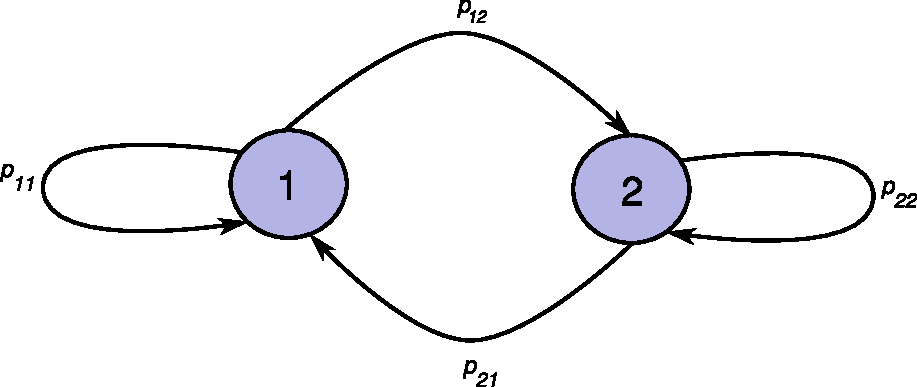
\includegraphics[scale=0.65]{Figures/transitions.pdf}
\caption{\it A transition diagram for a Markov Chain with two possible states.
The states (which correspond to hypotheses in Bayesian inference) are drawn
as circles labelled ``1'' and ``2''. When the algorithm is in a particular state
(e.g. State 1), and we apply one step of the Metropolis algorithm,
the probability it will be in State 1 is $p_{11}$ and the probability it
will be in State 2 is $p_{12}$.
MCMC works by making it easy to move into states with high
posterior probability, and hard to move out of them.
\label{fig:transitions}}
\end{center}
\end{figure}

\section{The Steady-State Distribution of a Markov Chain}
Once we have the transition matrix, we can work out the {\it steady state
distribution} of the Markov chain. Imagine, instead of starting the MCMC
from an arbitrary initial state, you have a probability distribution for the
initial state. After applying one iteration of the Metropolis algorithm, the
probability distribution for the updated state will usually be different from
the probability distribution for the initial state.

However, one special probability distribution, called the {\it steady state
distribution}, does not change after you apply an MCMC update. If your initial
point was drawn from the steady state distribution, then subsequent points will
also be drawn from the steady state distribution. In MCMC the steady state
distribution should be the same as the posterior distribution.

Imagine we are using MCMC on our two-state problem, and our initial position
is State 1 with probability $v_1$ and State 2 with probability $v_2$. What
is the probability of being in State 1 at the next iteration? There are two
ways for that to happen: by starting in State 1 and then making a transition
from $1\to 1$, or by starting in State 2  and making a transition from $2\to 1$.
The total probability is then:
\begin{eqnarray}
P(\textnormal{State 1 after iteration}) &=& v_1p_{11} + v_2p_{21}.
\end{eqnarray}
Similarly for State 2:
\begin{eqnarray}
P(\textnormal{State 2 after iteration}) &=& v_1p_{12} + v_2p_{22}.
\end{eqnarray}
If $v_1$ and $v_2$ happened to be the steady state distribution, then these
probabilities would also be $v_1$ and $v_2$. This gives us two simultaneous
equations
\begin{eqnarray}
v_1 &=& v_1p_{11} + v_2p_{21}\\
v_2 &=& v_1p_{12} + v_2p_{22}
\end{eqnarray}
which can also be written in matrix form as $\mathbf{v}\mathbf{P} = \mathbf{v}$
where $\mathbf{v} = \left(v_1, v_2\right)$ and $\mathbf{P}$ is the transition
matrix\footnote{Mathematics students might recognise this equation, which says
$\mathbf{v}$ is the left-eigenvector of $\mathbf{P}$, with eigenvalue 1.
An alternative is to write the stationary distribution as a column vector and
use $\mathbf{P}^T\mathbf{v} = \mathbf{v}$.}.
These two simultaneous equations can be solved for $v_1$ and $v_2$.
However there is a third constraint, that is $v_1 + v_2 = 1$. Since there
are three equations but two unknowns, it seems like the problem might be
``over-determined'', but that is not actually the case because the transition
matrix rows are not all linearly independent.
It is left as an exercise for the reader to show the steady state
distribution for our Markov chain (Equation~\ref{eq:p_matrix}) is in fact
equal to the posterior distribution, so
$\mathbf{v} = \left(\frac{1}{3}, \frac{2}{3}\right)$.

\section{Tactile MCMC}
In class we will do ``Tactile MCMC'', which is an implementation of the
Metropolis algorithm using coins and dice instead of the random number generators
provided in computer software such as R. This is a good way to get a feel for
the flow of MCMC algorithms.

In STATS 331, when we want to use MCMC in practice, we will use the JAGS program
rather than using Metropolis directly. JAGS is a general purpose MCMC program
which allows you to solve fairly complex problems without a large amount of
programming.
